\documentclass[11pt]{article}
\newcommand{\thetitle}{HYPERION Memo \#3: Testing the Radio Environment in 
Rangely, CO}
\newcommand{\theauthor}{Kara Kundert and Raj Biswas}
\newcommand{\theauthorsemail}{kkundert@berkeley.edu, rbiswas@berkeley.edu}
\newcommand{\thedate}{September 2017}
% the following controls some aspects of how the text is displayed on the page
\setlength{\textwidth}{6.5in}
\setlength{\textheight}{8.25in}
\setlength{\oddsidemargin}{0in}

% set up the page headers and footers
\usepackage{fancyhdr}
    \pagestyle{fancy}
    \lhead{\sffamily\slshape\small\thetitle}
    \rhead{\sffamily\small\theauthor}
    \cfoot{\sffamily\slshape\small\thepage}

% support display of graphics
\usepackage{graphicx}

% the following control some aspects of how paragraphs are displayed
\parindent=0pt
\parskip=2ex

% import library of technical symbols
\usepackage{amsmath,amssymb,latexsym}

% import bibliography tools
\usepackage{natbib}
\citestyle{aa}

\begin{document}
% print the title in san-serif font, in bold, in huge characters
\title{
    \sffamily\bfseries\huge
    \thetitle \\
}
% print the author in san-serif font
\author{
    \sffamily\theauthor \\
    \sffamily\theauthorsemail
}
\date{\thedate}
\maketitle
\sloppy

\section{Introduction}

This memo lays out the results of some initial radio environment testing in and 
around Rangely, Colorado. It also aims to lay out some analysis of what these 
results mean for the HYPERION instrument and suggests some new ideas for 
mitigation of environmental factors.

\section{Background and Theory}

One aspect of the HYPERION instrument that has yet to be finalized is its 
location -- where the instrument will be deployed to do the science it is 
designed to accomplish. Since its inception, there has been frequent discussion 
of using a site near Rangely, Colorado -- a tiny town in northwestern Colorado, 
far removed from most typical sources of radio transmission and peppered with 
convenient topology. With low RFI and a somewhat quieter radio sky, it seemed 
like an ideal candidate in theory. So, we put it to the test -- what does the 
radio environment around Rangely actually look like in the HYPERION frequency 
band?  And, assuming it's a good starting point, how can we optimize it to our 
peculiar needs?

To answer these questions, a series of three tests were conducted: one in the 
driveway of Aaron Parsons' parents house, one up a box canyon with limited N-EW 
exposure a short drive northeast, and another box canyon with limited exposure 
in all directions about 15 miles southwest. This changing directional exposure 
allowed us to begin investigating the effects of geological structure on the 
radio environment -- in particular, to see if rock formations around our 
antennas could serve as attenuators of ground-based sources of RFI. 

In each of these tests, a broadband dipole was hooked up to the FieldFox 
spectrum analyzer and used to record all that it picked up in a given frequency 
band (either 80-110 MHz or 0-300 MHz). Each spectra held 1001 points and was 
averaged for approximately 1 minute, collecting a maximum, minimum, and average 
spectrum for each recording.

\citep{pritchard-loeb2010}

\subsection{Receiver Noise and System Temperature}

In order to determine the overall system temperature of the Rangely, CO 
deployment system, we will first need to know the receiver noise temperature, 
$T_{rx}$, i.e.  the noise that would be added at the amplifier's input in order 
to account for the added noise observed following amplification. However, it 
would be too easy for the manufacturer's to simply provide $T_{rx}$, so instead 
we'll start from a noise figure $NF$ instead. Using 
Eq.~\eqref{eq:noise-figure}, we can calculate the noise factor $F$. For a 
single amplifier, we can then find the noise temperature using 
Eq.~\eqref{eq:noise-temp} with $T_0$ typically being set to a room temperature 
value of 290 K.

\begin{equation}
    \label{eq:noise-figure}
    NF = 10 \log_{10}(F)
\end{equation}

\begin{equation}
    \label{eq:noise-temp}
    F = \frac{T_0 + T}{T_0}
\end{equation}

In the case of the Rangely testing, two amplifiers were used in a chain. In 
this scenario, a final equation is needed to calculate the full receiver noise 
temperature, which accounts for the gain of the first amplifier on the effect 
of the amplifier noise contributions of the second amplifier. 

\begin{equation}
    \label{eq:receiver-temp}
    T_{rx} = T_1 + \frac{T_2}{g_1}
\end{equation}

The Rangely signal chain featured two identical amplifiers, each with a noise 
factor $NF = 11$ dB and a gain $g = 23$ dB. This led to a final receiver 
temperature of 3377 K across the band.

Ideally, we would like for our overall system temperature $T_{sys} = T_{rx} + 
T_{sync}$ to be dominated by a known term, such as the galactic synchrotron 
emission, $T_{sync}$.  

\begin{equation}
    \label{eq:sync-temp}
    T_{sync}(\nu) = T_{sync}(\textrm{150 MHz}) \left(\frac{\nu}{\textrm{150 
    MHz}}\right)^{-\beta}
\end{equation}

With the receiver temperature calculated in Eq.~\eqref{eq:receiver-temp} and 
the sky temperature calculated with Eq.~\eqref{eq:sync-temp}, we can find the 
difference between the total system temperature and the known sky temperature 
using Eq.~\eqref{eq:dB-to-sky}.

\begin{equation}
    \label{eq:dB-to-sky}
    \textrm{dB} = 10 \log\left(\frac{T_{sys}}{T_{sync}}\right)
\end{equation}

From this, we find that the system temperature $T_{sys}$ is approximately 5 dB 
brighter than the sky temperature $T_{sync}$ at 70 MHz. This indicates that the 
receiver system used during this round of testing will be inadequate for 
observations, as it will be difficult to properly calibrate the system with 
such a high level of noise being generated by our system.

\begin{figure}
    \begin{center}
    \includegraphics[width=\linewidth]{/home/kara/src/python/berkeley/plotters/noise_floor_rangely.png}
    \end{center}
    \caption{
        In this figure, we can see how the receiver temperature contributed to 
        the overall system. Ideally, we would like to be able to lower the 
        system temperature to the point where the synchrotron sky is the main 
        term across the band. However, as is evident above, the receiver chain 
        used in this particular testing trip introduced about 3400 K in noise 
        temperature, drowning out all but the absolute lowest frequencies of 
        the synchrotron sky. All in all, the synchrotron sky is approximately 5 
        dB down from the overall system temperature at 70 MHz.  In future 
        testing, we will need to develop a lower temperature signal chain to 
        mitigate this effect.
    }
    \label{fig:noise-floor}
\end{figure}


\section{Method}


\section{Data and Analysis}

\begin{figure}
    \begin{center}
    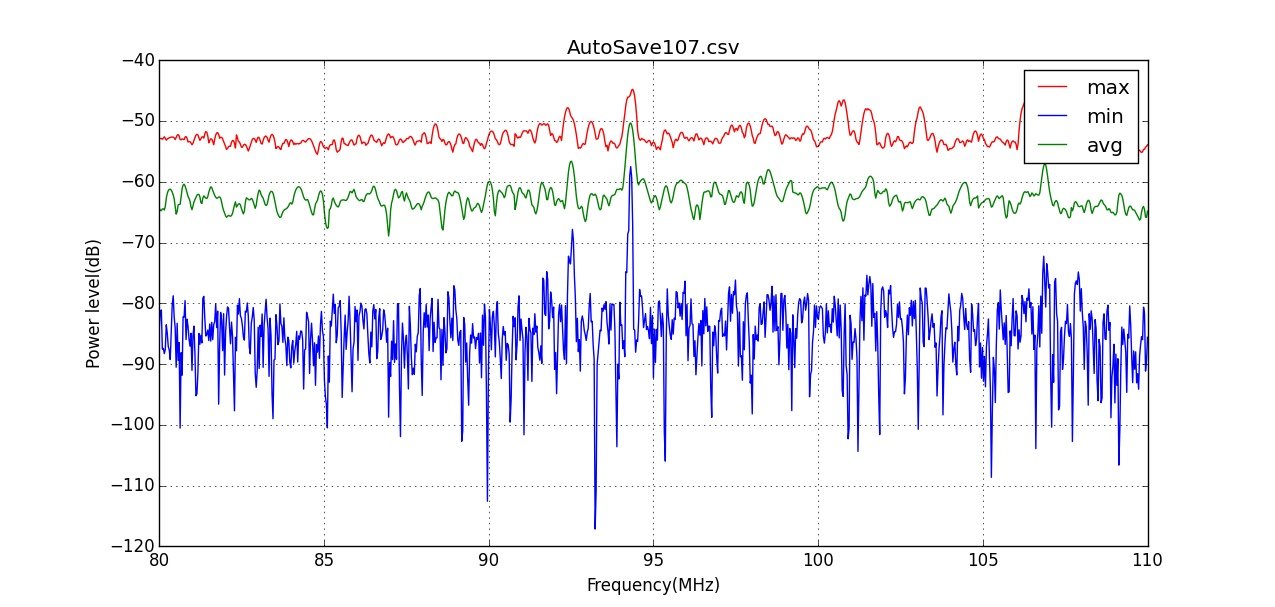
\includegraphics[width=\linewidth]{/home/kara/documents/hyperion/memos/memo3figs/107.jpeg}
    \end{center}
    \caption{
        Pictured above is the radio environment from 80-110 MHz as measured 
        from the creek bed in the box canyon off of Cottonwood Road, 
        approximately 15 miles southwest of Rangely.
    }
    \label{fig:107}
\end{figure}

\section{Conclusions}


\bibliography{hyperion}{}
\bibliographystyle{apj}

\end{document}





